\documentclass{article}
\usepackage[utf8]{inputenc}
\usepackage{authblk}
\usepackage{graphicx} % Lib de importar e tratar imagem
\usepackage[english,brazil]{babel} % Manter dois idiomas
\usepackage{fancyhdr} % Configuração das paginas
\usepackage{float}
\usepackage{xcolor}
\usepackage{titlesec}
\usepackage{background} % Componente de Watermark
\usepackage{hyperref}
\usepackage{verbatim}
\usepackage[a4paper, left=2cm, right=2cm]{geometry}
\usepackage[most]{tcolorbox}

\newcommand{\shellcmd}[1]{\\\indent\indent\texttt{\footnotesize\# #1}\\}

% Definir as características do hyperlink
\hypersetup{
    colorlinks=true,
    linkcolor=blue,
    filecolor=magenta,      
    urlcolor=cyan,
    pdftitle={Overleaf Example},
    pdfpagemode=FullScreen,
}

%Função para diminuir tamanho da fonte
\newcommand{\changefont}{%
    \fontsize{9}{12}\selectfont
}

%Document Layout Config
\pagestyle{fancy}
\setlength\headheight{26pt}
\setlength\parindent{0pt}
\fancyhf{}

% Header Config
\fancyhead[RO]{Autoridade Certificadora}
\fancyhead[LO]{\includegraphics[width=0.7cm]{Logo.png}}

% Footer Config
\renewcommand{\footrulewidth}{0.4pt} % Inserir linha no final da pagina "pre-footer"
\fancyfoot[RO]{\includegraphics[width=0.7cm]{Logo.png}}

%Document Specification
\title{Infraestrutura de Chaves Públicas (PKI)}
\author{senhasegura}
\affil{Departamento de Segurança e Inovação - SEGi9}
\date{}
\graphicspath{ {img/} }

%Capa
\begin{document}
\NoBgThispage % Ignorar background na capa
\maketitle
\begin{center}

\includegraphics{logo.png}
\end{center}
\begin{center}
\textbf{\LARGE \\PÚBLICO}
\end{center}
\pagenumbering{gobble} % Não contar como página a capa
\pagebreak

% Background a partir da segunda pagina
\backgroundsetup{contents=
\includegraphics{logo.png}, scale=1.5, opacity=0.15, angle=0} % marca d'agua

%Resumo Executivo
\section*{\centering{Resumo Executivo}}
\vspace*{\fill}
\large{Este texto tem como objetivo o de descrever os principais conceitos e funcionamento de uma Infraestrutura de Chaves Públicas (PKI).}
\vspace*{\fill}
\fancyfoot[CO]{senhasegura\\ \changefont Qualquer reprodução ou distribuição é estritamente proibida sem a aprovação prévia por escrito da empresa MT4.}
\pagebreak

%Sumario
\tableofcontents
\pagebreak

%Texto
\fancyfoot[CO]{\thepage\\\changefont Qualquer reprodução ou distribuição é estritamente proibida sem a aprovação prévia por escrito da empresa MT4.}
\pagenumbering{arabic}

%Página
\section{Princípios}

A segurança da informação é um campo fundamental no mundo digital atual, onde a proteção dos dados e informações é essencial para a manutenção da privacidade e a confiabilidade das operações.\\
Dentro deste contexto, existem quatro pilares importantes que sustentam a segurança da informação: Confidencialidade, Integridade e Autenticidade. Esses pilares são fundamentais para garantir a proteção adequada dos dados e a confiança nas transações e comunicações. A seguir, vamos explorar cada um desses conceitos:

\begin{itemize}
	\item Confidencialidade
	\item Integridade
	\item Autenticidade
\end{itemize}

\pagebreak

% Página
\section{Confidencialidade}

A Confidencialidade refere-se à garantia de que as informações são acessíveis apenas por pessoas autorizadas. Em outras palavras, é a proteção contra a divulgação não autorizada de dados. Este pilar é essencial para manter a privacidade dos dados pessoais e sensíveis, como informações financeiras, médicas ou estratégicas de uma organização. Técnicas de criptografia são amplamente utilizadas para garantir a confidencialidade, assegurando que, mesmo que os dados sejam interceptados, eles não possam ser lidos ou compreendidos por indivíduos não autorizados.

\subsection{Algoritmo Assimétrico}

O algoritmo de criptografia assimétrica é uma técnica fundamental no campo da segurança e criptografia. Diferente dos algoritmos de criptografia simétrica, que utilizam a mesma chave para criptografar e descriptografar os dados, os algoritmos assimétricos usam um par de chaves: uma \textbf{chave pública(KPu)} e uma \textbf{chave privada(KPr)}. Vamos explorar o funcionamento desse algoritmo através dos personagens Alice, Bob e Eva exemplificado pela Figura \ref{fig:algoritmo_assimetrico}.

\begin{figure}[H]
	\centering
	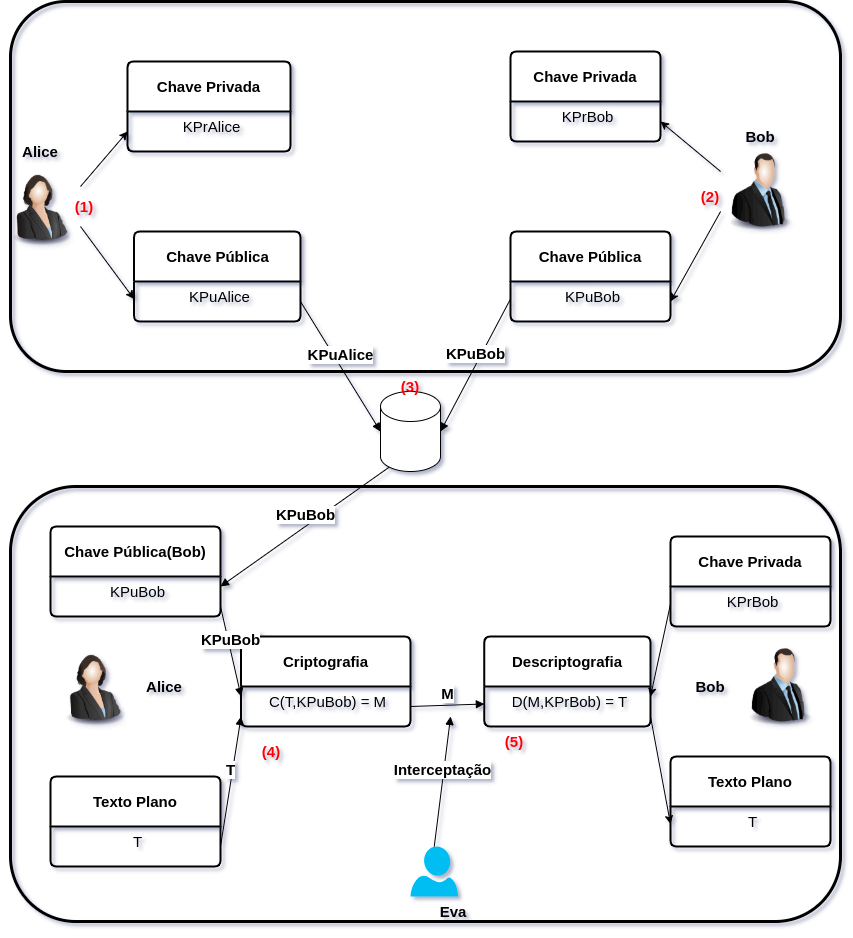
\includegraphics[scale=0.45]{algoritmo_assimetrico.png}
	\caption{Funcionamento do algoritmo de criptografia assimétrico}
	\label{fig:algoritmo_assimetrico}
\end{figure}

\pagebreak

%Página
\section{Integridade}

A Integridade diz respeito à precisão e consistência das informações ao longo de seu ciclo de vida. Este pilar assegura que os dados não sejam alterados de forma indevida, seja por erros acidentais ou por ações maliciosas. A integridade é mantida através de mecanismos de verificação, como somas de verificação, assinaturas digitais e funções de hash. Esses métodos permitem que qualquer alteração nos dados seja detectada, garantindo que a informação recebida é exatamente a mesma que foi enviada originalmente, sem modificações não autorizadas.
\subsection{Hash}

Um hash é uma função que transforma uma entrada de dados (que pode variar de alguns bytes a grandes volumes de dados) em uma saída de tamanho fixo, geralmente representada como uma sequência de caracteres alfanuméricos. Esta transformação é determinística, o que significa que a mesma entrada sempre produzirá a mesma saída.\\

Alguns exemplos de algoritmos hash populares incluem a família de algoritmos SHA-2 (Secure Hash Algorithm 2), que inclui SHA-224, SHA-256, SHA-384 e SHA-512. Os algoritmos SHA-2 produzem hashes de diferentes tamanhos, sendo o SHA-256 e o SHA-512 os mais comuns, gerando valores de 256 e 512 bits, respectivamente.\\

A Figura \ref{fig:hash} exemplifica a utilização do algoritmo de hash para verificar a integridade de uma informação enviada de \textbf{Bob} para \textbf{Alice}.\\

\begin{figure}[H]
	\centering
	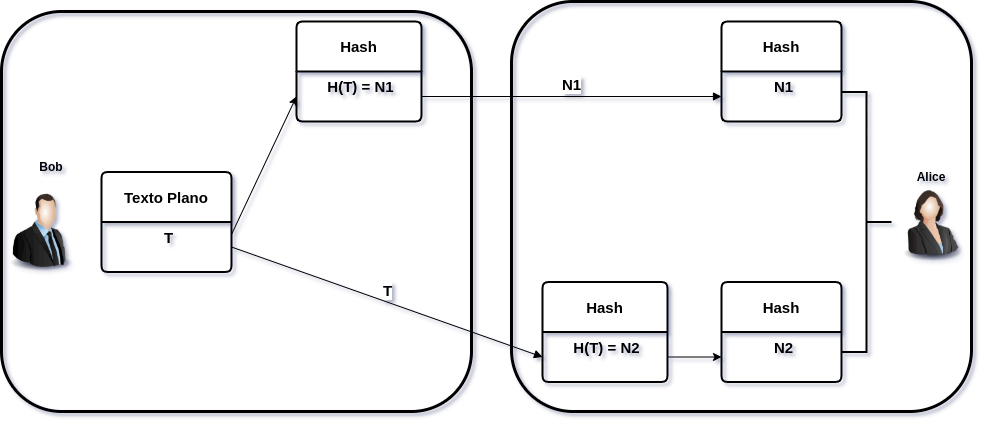
\includegraphics[scale=0.45]{hash.png}
	\caption{Funcionamento do processo de utilização do algoritmo Hash}
	\label{fig:hash}
\end{figure}

Inicialmente, \textbf{Bob} executa o algoritmo de hash sobre a mensagem e obtém o que normalmente é chamado de resumo. Tanto a mensagem quanto o resumo são enviados para \textbf{Alice}. \textbf{Alice} gera novamente o algoritmo de hash sobre a mensagem e compara o resultado do hash com o hash que foi enviado inicialmente por \textbf{Bob}. Se por acaso os valores forem iguais, então isso indica que não houve nenhum tipo de alteração na mensagem.\\

\pagebreak

% Página
\section{Autenticidade}

A Autenticidade está relacionada à verificação da identidade das partes envolvidas na comunicação e à garantia de que a origem das informações é confiável. Este pilar garante que as entidades (pessoas, sistemas ou dispositivos) sejam quem dizem ser e que as informações provenientes dessas entidades sejam genuínas. Métodos de autenticação, como senhas, certificados digitais e autenticação de dois fatores, são utilizados para validar a identidade e estabelecer a confiança entre as partes. A autenticidade é crucial para prevenir fraudes e assegurar a legitimidade das transações eletrônicas.

\subsection{Assinatura Digital}

A assinatura digital é um mecanismo de segurança criptográfica fundamental para garantir a integridade e a autenticidade das informações transmitidas digitalmente.\\

A assinatura digital utiliza algoritmos de \textbf{criptografia assimétrica} para garantir que uma mensagem ou documento não tenha sido alterado desde que foi assinado e que realmente foi enviado pelo remetente.\\

A Figura \ref{fig:assinatura} exemplifica o algoritmo de assinatura digital. Neste exemplo, Alice deseja enviar uma menagem para Bob e Alice deseja garantir que Bob possa verificar a autenticidade da mensagem.

\begin{figure}[H]
	\centering
	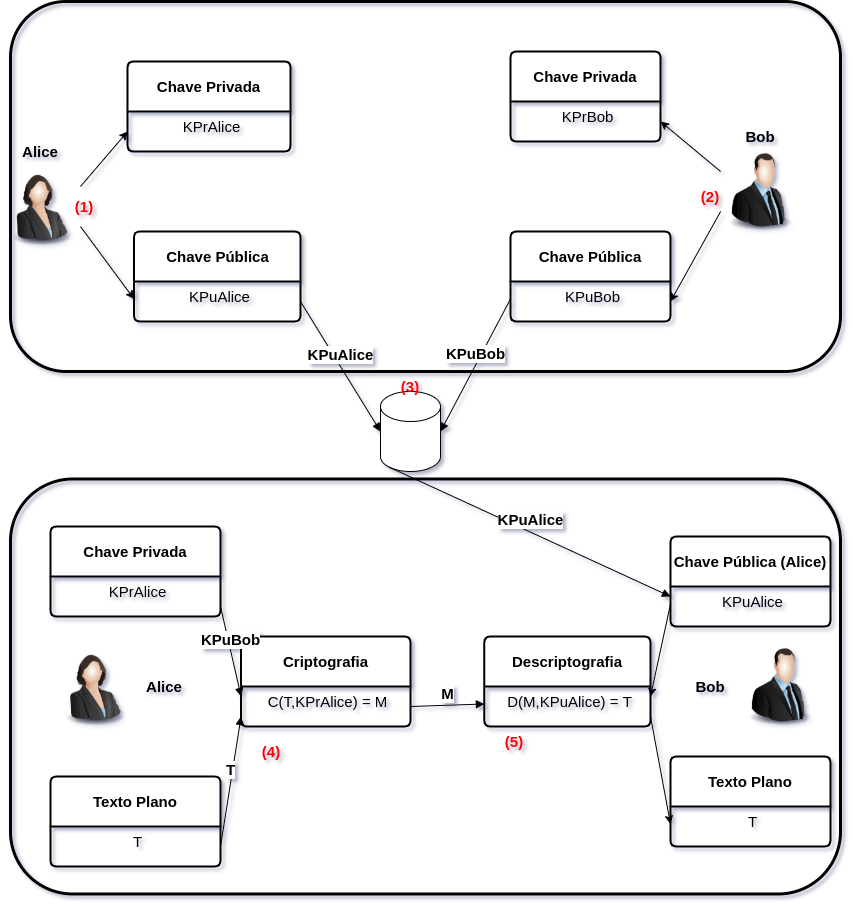
\includegraphics[scale=0.45]{assinatura.png}
	\caption{Funcionamento do processo de Assinatura Digital}
	\label{fig:assinatura}
\end{figure}

\pagebreak

%Página
\section{Autoridade de Certificação (CA)}

\subsection{O que é}

Uma Autoridade de Certificação (CA, do inglês Certificate Authority) é uma entidade confiável que emite certificados digitais. Esses certificados são usados para verificar a identidade de uma entidade (pessoa, organização ou dispositivo) e para estabelecer a confiança nas comunicações digitais. A CA desempenha um papel crucial na infraestrutura de chave pública (PKI, do inglês Public Key Infrastructure), que é usada para proteger transações e comunicações na internet.

\subsection{Funções Principais de uma CA}

\begin{itemize}
	\item \textbf{Emissão de Certificados Digitais: }A principal função de uma CA é emitir certificados digitais. 
	\item \textbf{Verificação de Identidade: }Antes de emitir um certificado, a CA verifica a identidade da entidade que solicita o certificado.
	\item \textbf{Assinatura de Certificados: }A CA assina digitalmente o certificado usando sua chave privada, garantindo que o certificado não tenha sido adulterado e que a identidade foi verificada pela CA.
	\item \textbf{Gestão de Certificados: }A CA também gerencia o ciclo de vida dos certificados.
\end{itemize}

\pagebreak

%Página
\section{Hierarquia de CAs}

O diagrama na Figura \ref{fig:ca} ilustra a hierarquia entre as CAs, incluindo a CA Root, a CA Intermediária e o Usuário Final. Cada um desses elementos possui características e funcionalidades específicas, que serão detalhadas a seguir.

\begin{figure}[H]
	\centering
	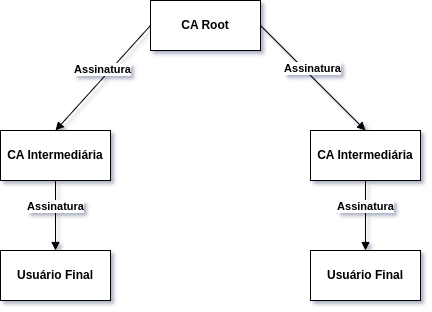
\includegraphics[scale=0.63]{ca.png}
	\caption{Hierarquia de CAs}
	\label{fig:ca}
\end{figure}

\subsection{Autoridade de Certificação (CA) Root}

Uma \textbf{Autoridade de Certificação (CA) Root} é a entidade central em uma infraestrutura de chave pública (PKI) que emite os primeiros certificados digitais, criando a base para a cadeia de confiança que valida identidades digitais na internet e em outros sistemas de comunicação segura. A CA Root emite e valida os certificados digitais, que são utilizados para autenticar a identidade de usuários, dispositivos ou servidores. Estes certificados garantem que a comunicação entre duas partes seja segura e confiável.\\

\subsection{Autoridade de Certificação (CA) Intermediária}

Uma \textbf{Autoridade de Certificação (CA) Intermediária} é uma entidade que emite certificados digitais em nome de uma Autoridade de Certificação Raiz (CA Raiz). Ela atua como um intermediário entre a CA Raiz, que é altamente confiável e segura, e os usuários finais ou servidores que recebem os certificados.\\

\subsection{Usuário Final}

Dentro de uma estrutura de Infraestrutura de Chave Pública (PKI) e Autoridade Certificadora (CA), o \textbf{Usuário Final} refere-se à entidade que utiliza certificados digitais para realizar atividades seguras, como autenticação, assinatura digital ou criptografia de dados. Esse usuário final pode ser uma pessoa, um dispositivo, um serviço ou uma aplicação.\\

\pagebreak

%Página
\section{Prático}

\begin{enumerate}
	\item CA Root / CA Intermediária - Estrutura de Diretórios
	\begin{tcolorbox}[width=\textwidth]
	{\footnotesize
		\begin{verbatim}
			$ mkdir -p /root/ca/root-ca/{certs,crl,newcerts,private}
			$ mkdir -p /root/ca/intermediate-ca/{certs,crl,csr,newcerts,private}
			$ mkdir /root/ca/user-certs
			$ chmod 700 /root/ca/root-ca/private /root/ca/intermediate-ca/private
			$ touch /root/ca/root-ca/index.txt /root/ca/intermediate-ca/index.txt
			$ echo 1000 > /root/ca/root-ca/serial
			$ echo 1000 > /root/ca/intermediate-ca/serial
			$ echo 1000 > /root/ca/root-ca/crlnumber
			$ echo 1000 > /root/ca/intermediate-ca/crlnumber
		\end{verbatim}
	}
	\end{tcolorbox}

	\item CA Root - Configuração da CA Root (/root/ca/root-ca/openssl.cnf)
	\begin{tcolorbox}[width=\textwidth, enhanced, breakable]
	{\footnotesize
		\begin{verbatim}
			[ ca ]
			default_ca = CA_default
			
			[ CA_default ]
			dir               = /root/ca/root-ca
			certs             = $dir/certs
			crl_dir           = $dir/crl
			new_certs_dir     = $dir/newcerts
			database          = $dir/index.txt
			serial            = $dir/serial
			private_key       = $dir/private/root-ca.key.pem
			certificate       = $dir/certs/root-ca.cert.pem
			crlnumber         = $dir/crlnumber
			crl               = $dir/crl/root-ca.crl.pem
			crl_extensions    = crl_ext
			default_crl_days  = 30
			default_md        = sha256
			name_opt          = ca_default
			cert_opt          = ca_default
			default_days      = 3650
			preserve          = no
			policy            = policy_strict
			
			[ policy_strict ]
			countryName             = match
			stateOrProvinceName     = match
			organizationName        = match
			organizationalUnitName  = optional
			commonName              = supplied
			emailAddress            = optional
			
			[ req ]
			default_bits        = 4096
			distinguished_name  = req_distinguished_name
			string_mask         = utf8only
			default_md          = sha256
			prompt              = no
			
			[ req_distinguished_name ]
			countryName                     = BR
			stateOrProvinceName             = Sao Paulo
			localityName                    = Sao Paulo
			0.organizationName              = senhasegura
			organizationalUnitName          = IT Department
			commonName                      = My Root CA
			emailAddress                    = mt4@senhasegura.com
			
			[ v3_ca ]
			subjectKeyIdentifier = hash
			authorityKeyIdentifier = keyid:always,issuer
			basicConstraints = critical,CA:true
			keyUsage = critical, digitalSignature, cRLSign, keyCertSign
			
			[ v3_intermediate_ca ]
			subjectKeyIdentifier = hash
			authorityKeyIdentifier = keyid:always,issuer
			basicConstraints = critical,CA:true,pathlen:0
			keyUsage = critical, digitalSignature, cRLSign, keyCertSign
			
			[ crl_ext ]
			authorityKeyIdentifier=keyid:always
		\end{verbatim}
	}
	\end{tcolorbox}

	\item CA Intermediária - Configuração da CA Intermediária (/root/ca/intermediate-ca/openssl.cnf)
	\begin{tcolorbox}[width=\textwidth, enhanced, breakable]
	{\footnotesize
		\begin{verbatim}
			$ cat /root/ca/intermediate-ca/openssl.cnf

			[ ca ]
			default_ca = CA_default
			
			[ CA_default ]
			dir               = /root/ca/intermediate-ca
			certs             = $dir/certs
			crl_dir           = $dir/crl
			new_certs_dir     = $dir/newcerts
			database          = $dir/index.txt
			serial            = $dir/serial
			private_key       = $dir/private/intermediate-ca.key.pem
			certificate       = $dir/certs/intermediate-ca.cert.pem
			crlnumber         = $dir/crlnumber
			crl               = $dir/crl/intermediate-ca.crl.pem
			crl_extensions    = crl_ext
			default_crl_days  = 30
			default_md        = sha256
			name_opt          = ca_default
			cert_opt          = ca_default
			default_days      = 3650
			preserve          = no
			policy            = policy_loose
			
			[ policy_loose ]
			countryName             = match
			stateOrProvinceName     = match
			organizationName        = match
			organizationalUnitName  = optional
			commonName              = supplied
			emailAddress            = optional
			
			[ req ]
			default_bits        = 4096
			distinguished_name  = req_distinguished_name
			string_mask         = utf8only
			default_md          = sha256
			prompt              = no
			
			[ req_distinguished_name ]
			countryName                     = BR
			stateOrProvinceName             = Sao Paulo
			localityName                    = Sao Paulo
			0.organizationName              = senhasegura
			organizationalUnitName          = SEGi9
			commonName                      = My Intermediate CA
			emailAddress                    = segi9@senhasegura.com
			
			[ v3_intermediate_ca ]
			subjectKeyIdentifier = hash
			authorityKeyIdentifier = keyid:always,issuer
			basicConstraints = critical,CA:true,pathlen:0
			keyUsage = critical, digitalSignature, cRLSign, keyCertSign
			
			[ crl_ext ]
			authorityKeyIdentifier=keyid:always
			
			[ usr_cert ]
			basicConstraints = CA:FALSE
			nsCertType = client, email
			nsComment = "User Certificate"
			subjectKeyIdentifier = hash
			authorityKeyIdentifier = keyid,issuer
			keyUsage = critical, nonRepudiation, digitalSignature, keyEncipherment
			extendedKeyUsage = clientAuth, emailProtection
		\end{verbatim}
	}
	\end{tcolorbox}

	\item CA Root - Criar o Par de Chaves e Certificado da CA Root
	\begin{tcolorbox}[width=\textwidth]
	{\footnotesize
		\begin{verbatim}
			$ openssl genpkey -algorithm RSA -out /root/ca/root-ca/private/root-ca.key.pem \
			-pkeyopt rsa_keygen_bits:4096

			$ chmod 400 /root/ca/root-ca/private/root-ca.key.pem
			
			$ openssl req -config /root/ca/root-ca/openssl.cnf -key /root/ca/root-ca/private/root-ca.key.pem \
			-new -x509 -days 7300 -sha256 -extensions v3_ca -out /root/ca/root-ca/certs/root-ca.cert.pem

			$ chmod 444 /root/ca/root-ca/certs/root-ca.cert.pem
		\end{verbatim}
	}
	\end{tcolorbox}

	\item CA Intermediária - Criar o Par de Chaves da CA Intermediária
	\begin{tcolorbox}[width=\textwidth]
	{\footnotesize
		\begin{verbatim}
			$ openssl genpkey -algorithm RSA -out /root/ca/intermediate-ca/private/intermediate-ca.key.pem \
			-pkeyopt rsa_keygen_bits:4096

			$ chmod 400 /root/ca/intermediate-ca/private/intermediate-ca.key.pem
		\end{verbatim}
	}
	\end{tcolorbox}

	\item CA Intermediária - Criar a Solicitação de Certificado (CSR) da CA Intermediária
	\begin{tcolorbox}[width=\textwidth]
	{\footnotesize
		\begin{verbatim}
			$ openssl req -config /root/ca/intermediate-ca/openssl.cnf -new -sha256 \
			-key /root/ca/intermediate-ca/private/intermediate-ca.key.pem \
			-out /root/ca/intermediate-ca/csr/intermediate-ca.csr.pem
		\end{verbatim}
	}
	\end{tcolorbox}

	\item CA Root / CA Intermediária - Assinar o Certificado da CA Intermediária com a CA Root
	\begin{tcolorbox}[width=\textwidth]
	{\footnotesize
		\begin{verbatim}
			$ openssl ca -batch -config /root/ca/root-ca/openssl.cnf -extensions v3_intermediate_ca \
			-days 3650 -notext -md sha256 -in /root/ca/intermediate-ca/csr/intermediate-ca.csr.pem \
			-out /root/ca/intermediate-ca/certs/intermediate-ca.cert.pem

			$ chmod 444 /root/ca/intermediate-ca/certs/intermediate-ca.cert.pem
		\end{verbatim}
	}
	\end{tcolorbox}

	\item CA Intermediária - Criar a Cadeia de Certificados
	\begin{tcolorbox}[width=\textwidth]
	{\footnotesize
		\begin{verbatim}
			$ cat /root/ca/intermediate-ca/certs/intermediate-ca.cert.pem /root/ca/root-ca/certs/root-ca.cert.pem > \
			/root/ca/intermediate-ca/certs/ca-chain.cert.pem

			$ chmod 444 /root/ca/intermediate-ca/certs/ca-chain.cert.pem
		\end{verbatim}
	}
	\end{tcolorbox}

	\item Usuário - Criar o Par de Chaves do Usuário Final
	\begin{tcolorbox}[width=\textwidth]
	{\footnotesize
		\begin{verbatim}
			$ openssl genpkey -algorithm RSA -out /root/ca/user-certs/user.key.pem -pkeyopt rsa_keygen_bits:2048

			$ chmod 400 /root/ca/user-certs/user.key.pem
		\end{verbatim}
	}
	\end{tcolorbox}

	\item Usuário - Criar a Solicitação de Certificado (CSR) do Usuário Final
	\begin{tcolorbox}[width=\textwidth]
	{\footnotesize
		\begin{verbatim}
			$ openssl req -new -sha256 -key /root/ca/user-certs/user.key.pem \
			-subj "/C=BR/ST=Sao Paulo/L=Sao Paulo/O=senhasegura/OU=Users/CN=usuario.exemplo" \
			-out /root/ca/user-certs/user.csr.pem
		\end{verbatim}
	}
	\end{tcolorbox}

	\item Usuário - Assinar o Certificado de Usuário Final com a CA Intermediária
	\begin{tcolorbox}[width=\textwidth]
	{\footnotesize
		\begin{verbatim}
			$ openssl ca -batch -config /root/ca/intermediate-ca/openssl.cnf -extensions usr_cert -days 375 -notext \
			-md sha256 -in /root/ca/user-certs/user.csr.pem -out /root/ca/user-certs/user.cert.pem

			$ chmod 444 /root/ca/user-certs/user.cert.pem
		\end{verbatim}
	}
	\end{tcolorbox}

	\item Usuário - Verificar a Cadeia de Certificados
	\begin{tcolorbox}[width=\textwidth]
	{\footnotesize
		\begin{verbatim}
			$ openssl verify -CAfile /root/ca/intermediate-ca/certs/ca-chain.cert.pem \
			/root/ca/user-certs/user.cert.pem
		\end{verbatim}
	}
	\end{tcolorbox}

\end{enumerate}

\pagebreak

%Copyright
\vspace*{\fill}
\begin{flushright}
	\underline{\textit{Copyright}}\\
	All rights reserved to MT4 Tecnologia LTDA.\bigskip

	\underline{\textit{Propósito deste documento}}\\
	Infraestrutura de Chaves Públicas (PKI)\bigskip
	
	\underline{\textit{MT4 Tecnologia Ltda.}}\\
	Rua Joaquim Antunes, 767 – Pinheiros – São Paulo\\
	Phone: +55 11 3065-7070\\
	\url{www.mt4.com.br}\\
	\href{mailto:support@senhasegura.com}{support@senhasegura.com}\\
\end{flushright}

\end{document}
